\chapter{Introdução}[Introdução]
O crescimento tecnológico atinge todas as áreas disponíveis no mundo permitindo uma mudança radical em todos os setores, nas bibliotecas não poderia ser diferente.

Antigamente utilizavam-se documentos manuais como carteirinhas, carimbos e outros dispositivos que demandam um certo tempo para solicitar um empréstimo de um livro e sua devolução. Depois, com a criação de computadores e o desenvolvimento de programas referentes ao armazenamento de dados, foi possível diminuir a quantidade de tempo perdido para o empréstimo e sua devolução, porém, ainda assim não é considerado um sistema eficaz pois demanda uma quantidade de tempo até a solicitação do livro e a procura nas prateleiras. No caso de empréstimo existe o enfrentamento de filas na devolução, sem levar em consideração outros aspectos de caráter burocrático com relação a entrada e saída da biblioteca, e outros fatores.

Para solucionar esse problema, o presente trabalho visa a construção de um dispositivo que tem a finalidade de entregar o livro solicitado do acervo ao usuário. A devolução do livro ao seu lugar específico sem que o usuário necessite entrar na biblioteca somente para alugar ou devolver um livro é uma das vantagens da biblioteca automatizada. Isso promoverá a melhoria da atividade facilitando tanto o trabalho do bibliotecário quanto a vida de um estudante.

A partir disso, será desenvolvido um protótipo denominado Bibliotech baseado nos conhecimentos adquiridos durante todo curso referente a todas as engenharias e a partir de um levantamento bibliográfico.

\section{Contexto}

O papel de uma biblioteca é a difusão de informações para os usuários. Para atingir essa finalidade, é necessário promover um sistema onde a relação de informação e usuário seja aperfeiçoada. Contudo, é necessária uma automatização sistemática, prática e acessível para que o usuário não se desgaste na busca ao acervo disponível e na organização do mesmo. 

A primeira biblioteca foi criada antes de Cristo a partir do armazenamento de uma grande quantidade de tabuletas nas quais se localizavam uma escrita cuneiforme pois era produzida através de objetos denominados “cunhas”. A partir de então, bibliotecas acompanham o desenvolvimento tecnológico no qual pode ser identificado através de atividades automatizadas onde pode facilitar o trabalho dos bibliotecários e auxiliar os estudantes em atividades como: devolução e empréstimo de livro e consulta no banco de dados.

Essa automatização pode substituir o trabalho humano em muitas tarefas comuns no dia a dia. Não é mais necessário procurar um livro ou um documento que deseja em diversas fichas pois já existe um banco de dados disponível com um grande armazenamento de autores, títulos e periódicos que podem ser acessados livremente, inclusive do seu próprio dispositivo.

Hoje se encontra disponível na maioria das bibliotecas somente uma automatização referente ao banco de dados, e o usuário ainda enfrenta um desgaste referente à procura de livro em prateleiras, enfrentamento de filas para retirada e devolução do livro e um grande trabalho monótono por parte do bibliotecário em devolver uma grande quantidade de livros às prateleiras. Por isso, já se fala em um sistema automatizado que retire e reponha os exemplares necessários de um local sem a influência de um humano. 

Pensa-se em um dispositivo no qual o bibliotecário solicita um exemplar em um catálogo virtual. Em seguida, o livro será localizado e levado até ele por meio de um robô. O bibliotecário terá somente a finalidade de registrar esse empréstimo e entregar para o solicitante.  A devolução seguirá o mesmo procedimento, após o livro ser depositado em uma caixa, o bibliotecário permitirá que o robô faça a destinação correspondente ao livro.

O maior benefício será o aprimoramento da biblioteca que promoverá um bem-estar tanto para o usuário quanto para o bibliotecário em relação ao controle do acervo, levantamentos bibliográficos e serviços de empréstimos e devolução do livro. 

\section{Problema}

\begin{figure}
\centering 
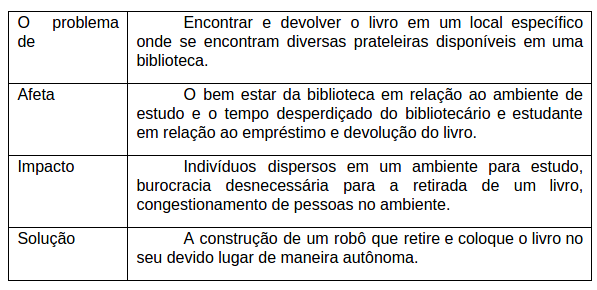
\includegraphics[scale=1]{tabela_1}
\end{figure}

\section{Justificativa}
O projeto tem a finalidade de desenvolver um produto a partir dos conhecimentos adquiridos durante o período acadêmico dos estudantes de engenharia aeroespacial, automotiva, eletrônica, energia e software. Foi definida a construção de um robô que tem a função de retirar e colocar livros em locais específicos quando solicitado. A importância desse equipamento é diminuir o congestionamento de pessoas no interior da biblioteca, problema que acaba atrapalhando os indivíduos que de fato, querem usar ao ambiente para os estudos.  Além do mais, pode poupar o tempo das pessoas que vão à biblioteca somente para a retirada de livros

\section{Objetivo}
O objetivo deste trabalho é construir um robô com a finalidade de localizar um livro desejado, retirar do seu local apropriado e colocá-lo no mesmo local quando este for devolvido à biblioteca.

\section{Objetivos Específicos}
\begin{itemize}
\item Desenvolver uma estrutura adequada.
\item Desenvolver um sistema de monitoramento e controle.
\item Implantar um sistema de alimentação adequado para garantir o funcionamento do dispositivo.
\item Definir e projetar um sistema embarcado.
\item Montar o robô através da integração entre estrutura, monitoramento e controle, alimentação e software. 
\end{itemize}
